\documentclass[border=4pt]{standalone}
% Preámbulo común de las figuras. Cada figura es un documento standalone
% que se compila a SVG con scripts/build_figures.sh
\usepackage[utf8]{inputenc}
\usepackage{amsmath}
\usepackage{tikz}
\usepackage[american, siunitx]{circuitikz}
\usetikzlibrary{arrows.meta,calc,decorations.pathmorphing,patterns}
\tikzset{
  >={Stealth[length=2.2mm]},
  eje/.style={->, thin},
  hilo/.style={thick},
}
% Paleta común: tonos medios legibles sobre fondo claro
\definecolor{azul}{RGB}{31,94,168}
\definecolor{rojo}{RGB}{192,57,43}
\definecolor{verde}{RGB}{39,128,73}
\definecolor{naranja}{RGB}{211,120,30}
\definecolor{morado}{RGB}{125,60,152}

\begin{document}
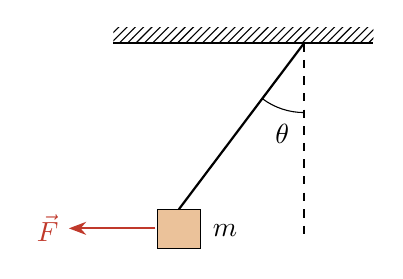
\begin{tikzpicture}[scale=1.1]
  \fill[pattern=north east lines] (-2.2,0) rectangle (0.8,0.18);
  \draw[thick] (-2.2,0) -- (0.8,0);
  \coordinate (O) at (0,0);
  \coordinate (L) at ({-2.4*sin(37)},{-2.4*cos(37)});
  \draw[hilo] (O) -- (L);
  \draw[dashed] (O) -- (0,-2.3);
  \draw (0,-0.8) arc[start angle=-90, end angle={-90-37}, radius=0.8];
  \node at (-0.25,-1.05) {$\theta$};
  \fill[naranja!45] ($(L)+(-0.25,-0.45)$) rectangle ($(L)+(0.25,0)$);
  \draw ($(L)+(-0.25,-0.45)$) rectangle ($(L)+(0.25,0)$);
  \draw[->, thick, rojo] ($(L)+(-0.27,-0.22)$) -- ++(-1.0,0) node[left]{$\vec{F}$};
  \node[right] at ($(L)+(0.28,-0.25)$) {$m$};
\end{tikzpicture}
\end{document}
